\subsection{Basic use of Sophus}
We have introduced the introductory knowledge of Lie algebra, and now it is time to consolidate what we have learned through practical exercises. Let's discuss how to manipulate Lie algebra in a program. In Lecture 3, we saw that Eigen provided geometry modules, but did not provide support for Lie algebra. A better Lie algebra library is the Sophus library maintained by Strasdat\footnote{The earliest proposed Lie algebra is Sophus Lie, which is named after him. }. The Sophus library supports $\mathrm{SO}(3)$ and $\mathrm{SE}(3)$, which are mainly discussed in this chapter. In addition, it also contains two-dimensional motion $\mathrm{SO}(2), \mathrm{SE} (2) $ and the similar transformation of $\mathrm{Sim}(3)$. It is developed directly on top of Eigen and we don't need to install additional dependencies. Readers can get Sophus directly from GitHub, or the Sophus source code is also available in the book's code directory slambook/3rdparty. For historical reasons, earlier versions of Sophus only provided double-precision Lie group/Lie algebra classes. Subsequent versions have been rewritten as template classes. Different precision Lie group/Lie algebra can be used in the Sophus of the template class, but at the same time it increases the difficulty of use. In the second edition of this book, we use the Sophus library of \textbf{with template}. The Sophus provided in the 3rdparty of this book is the \textbf{template} version, which should have been copied when you downloaded the code for this book. Sophus itself is also a cmake project. Presumably you already know how to compile the cmake project, so I won't go into details here. The Sophus library only needs to be compiled, no need to install it.

Let's demonstrate the SO(3) and SE(3) operations in the Sophus library:

\begin{lstlisting}[language=c++,caption=slambook/ch4/useSophus.cpp]
#include <iostream>
#include <cmath>
#include <Eigen/Core>
#include <Eigen/Geometry>
#include "sophus/se3.hpp"

Using namespace std;
Using namespace Eigen;

/// This program demonstrates the basic usage of sophus
Int main(int argc, char **argv) {
// Rotation matrix rotated 90 degrees along the Z axis
Matrix3d R = AngleAxisd(M_PI / 2, Vector3d(0, 0, 1)).toRotationMatrix();
// or quaternion
Quaterniond q(R);
Sophus::SO3d SO3_R(R); // Sophus::SO3d can be constructed directly from the rotation matrix
Sophus::SO3d SO3_q(q); // can also be constructed by quaternion
// Both are equivalent
Cout << "SO(3) from matrix:\n" << SO3_R.matrix() << endl;
Cout << "SO(3) from quaternion:\n" << SO3_q.matrix() << endl;
Cout << "they are equal" << endl;

// Use the logarithmic map to get its Lie algebra
Vector3d so3 = SO3_R.log();
Cout << "so3 = " << so3.transpose() << endl;
// hat is vector to antisymmetric matrix
Cout << "so3 hat=\n" << Sophus::SO3d::hat(so3) << endl;
// Relative, vee is the objection vector
Cout << "so3 hat vee= " << Sophus::SO3d::vee(Sophus::SO3d::hat(so3)).transpose() << endl;

// Update of the incremental disturbance model
Vector3d update_so3(1e-4, 0, 0); //assuming the update is so much
Sophus::SO3d SO3_updated = Sophus::SO3d::exp(update_so3) * SO3_R;
Cout << "SO3 updated = \n" << SO3_updated.matrix() << endl;

Cout << "*******************************" << endl;
// The same is true for SE(3) operations
Vector3d t(1, 0, 0); // translate 1 along the x axis
Sophus::SE3d SE3_Rt(R, t); // Construct SE(3) from R, t
Sophus::SE3d SE3_qt(q, t); // Construct SE(3) from q,t
Cout << "SE3 from R,t= \n" << SE3_Rt.matrix() << endl;
Cout << "SE3 from q,t= \n" << SE3_qt.matrix() << endl;
// The Lie algebra se(3) is a six-dimensional vector. For convenience, typedef is used first.
Typedef Eigen::Matrix<double, 6, 1> Vector6d;
Vector6d se3 = SE3_Rt.log();
Cout << "se3 = " << se3.transpose() << endl;
// Observe the output, you will find that in Sophus, the translation of se(3) is in front and the rotation is in the back.
// Same, there are two operators of hat and vee
Cout << "se3 hat = \n" << Sophus::SE3d::hat(se3) << endl;
Cout << "se3 hat vee = " << Sophus::SE3d::vee(Sophus::SE3d::hat(se3)).transpose() << endl;

// Finally, demonstrate the update
Vector6d update_se3; //update volume
update_se3.setZero();
Update_se3(0, 0) = 1e-4d;
Sophus::SE3d SE3_updated = Sophus::SE3d::exp(update_se3) * SE3_Rt;
Cout << "SE3 updated = " << endl << SE3_updated.matrix() << endl;

Return 0;
}
\end{lstlisting}

The result of this program output is 2.207, and the image is shown as \autoref{fig:trajectory-compare}. The reader also tries to remove the rotating part and only calculates the error of the translation part. For this example, we have actually helped the reader to do some pre-processing tasks, including time alignment of the trajectory and external parameter estimation. These contents have not been mentioned yet, and we will talk about it in future learning.

\begin{figure}[!ht]
	\centering
	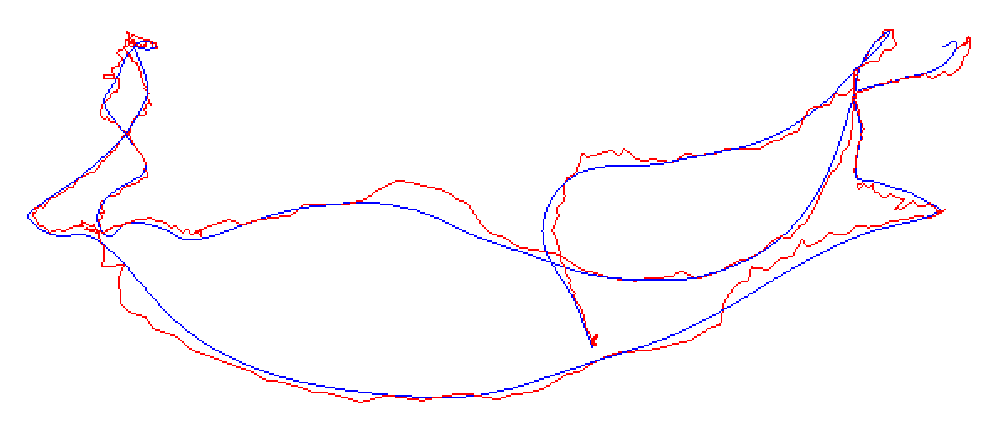
\includegraphics[width=1.0\textwidth]{chapter04/lieGroup/trajectory-compare.pdf}
	\caption{chapter04/calculates the error between the estimated trajectory and the real trajectory. }
	\label{fig:trajectory-compare}
\end{figure}